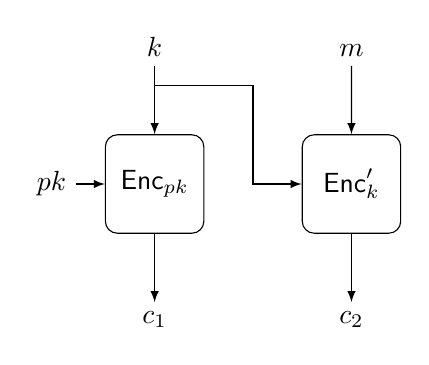
\begin{tikzpicture}
\node (f1) [minimum size=1.25cm,rounded corners=1ex,draw] {$\mathsf{Enc}_{pk}$};
\node (f2) at (2.5cm,0) [minimum size=1.25cm,rounded corners=1ex,draw] {$\mathsf{Enc}'_{k}$};
\draw[-latex] (0,1.5cm) node [above] {$k$} -- (f1);
\draw[-latex] (2.5,1.5cm) node [above] {$m$} -- (f2);
\draw[-latex] (-1cm,0) node [left] {$pk$} -- (f1);
\draw[-latex] (f1) -- +(0,-1.5) node [below] {$c_1$};
\draw[-latex] (f2) -- +(0,-1.5) node [below] {$c_2$};
\draw[-latex] (0,1.25) -| (1.25,0) -- (f2);
\end{tikzpicture}